% Requires graphicx. Keep these PNGs alongside the manuscript, or adjust paths.
% Existing bibliography key: AnchorProteinSketch.
% DRAFT: confirm crop/publication reuse permission before submission.
\begin{figure*}[t]
  \centering
  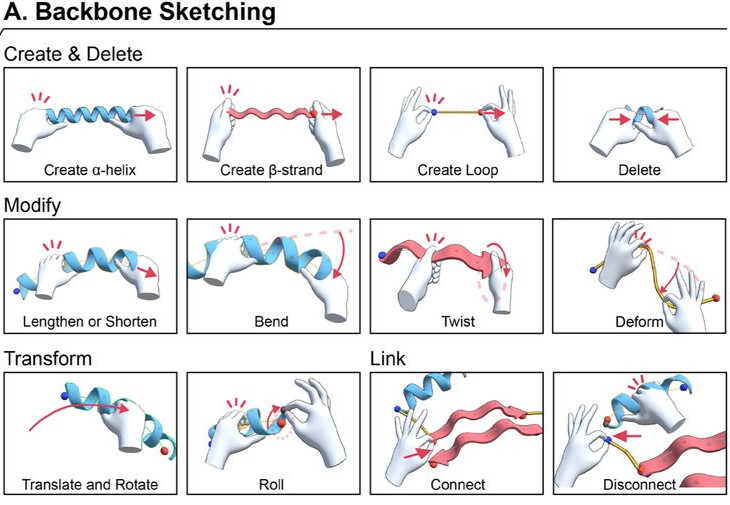
\includegraphics[width=0.64\textwidth]{figures/system-examples/proteinsketch_backbone_crop.png}\\[5pt]
  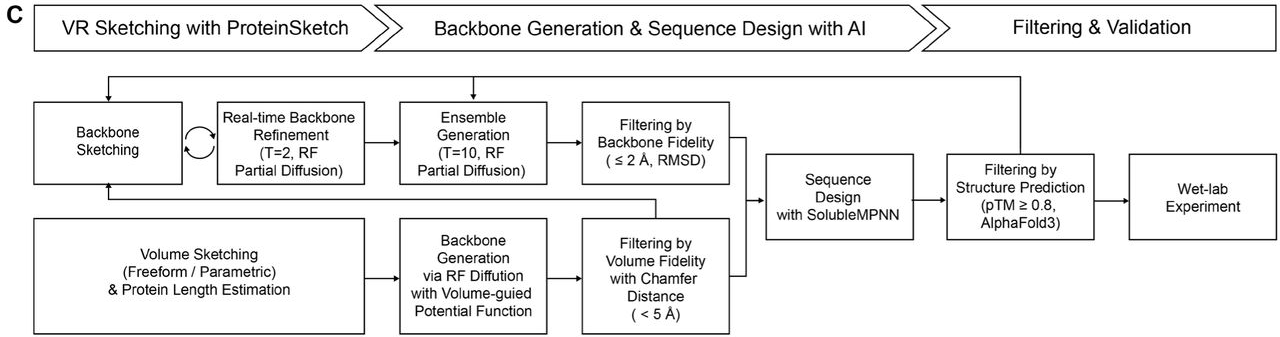
\includegraphics[width=\textwidth]{figures/system-examples/proteinsketch_workflow_crop.png}
  \caption{ProteinSketch connects spatial specification to generative protein design. (A) Two-handed gestures create, reshape, and connect secondary-structure elements in VR. (C) Backbone sketches and volumetric constraints feed computational refinement, generation, sequence design, and filtering. Scientists specify the desired geometry while computational models propose and evaluate candidate structures, linking Immersive and Algorithmic assistance within the design workflow. Selected panels cropped from Ma et al.~\cite{AnchorProteinSketch}, Fig.~1; original panel labels retained.}
  \label{fig:proteinsketch-workflow}
\end{figure*}
